\chapter{Terrain-following coordinates for ICONAM}

\section{Definition of the terrain following coordinate system}

For the nonhydrostatic formulation of the model equations we need the
divergence, gradient, and rotation operators in terrain following coordinates.
The problem we are faced with in our special case of the ICON grid is the lack
of boxes with quadrilateral faces, which are generally needed when considering
different coordinate systems, such as the contravariant and covariant systems
which are contragredient to each other. The proposal to overcome this problem
is thus to define quadrilateral boxes as base entities {\it additionally} to the
main triangular, quadrilateral or hexagonale/pentagonal grid boxes. This seems
unsuitable at first glance, but you will quickly appreciate the advantages of
this proceeding.

\begin{figure}[h]
%\begin{pdfdisplay}
\setlength{\unitlength}{0.5cm}
\begin{pspicture}(0,0)(0,0)
%Dreieck
\psset{unit=0.5cm}
\psset{fillstyle=solid}
\pspolygon[fillcolor=blue](0,0)(6,0)(3,1.7321)
\pspolygon[fillcolor=green](0,0)(3,1.7321)(3,5.1962)
\pspolygon[fillcolor=red](6,0)(3,1.7321)(3,5.1962)
\pspolygon[hatchcolor=blue,fillstyle=crosshatch](0,1.7321)(6,1.7321)(6,-1.7321)(0
, -1.7321)
\pspolygon[hatchcolor=green,fillstyle=hlines](1.5,-0.8660)(-1.5,0.8660)(1.5,
6.0622)(4.5 , 4.3301)
\pspolygon[hatchcolor=red,fillstyle=vlines](4.5,-0.8660)(7.5,0.8660)(4.5,
6.0622)(1.5 , 4.3301)
%Viereck
\psset{unit=0.5cm}
\pspolygon[fillstyle=none](9,0)(13,0)(13,4)(9,4)
\pspolygon[fillstyle=solid,fillcolor=blue](13,0)(11,2)(13,4)
\pspolygon[fillstyle=solid,fillcolor=red](9,4)(11,2)(13,4)
\pspolygon[fillstyle=solid,fillcolor=yellow](9,0)(11,2)(13,0)
\pspolygon[fillstyle=solid,fillcolor=green](9,0)(11,2)(9,4)
\pspolygon[fillstyle=hlines,hatchcolor=blue](11,0)(11,4)(15,4)(15,0)
\pspolygon[fillstyle=vlines,hatchcolor=red](9,2)(13,2)(13,6)(9,6)
%Seckseck
\psset{unit=0.5cm}
\pspolygon[fillstyle=none](18,3.4641016)(18,0)(21,-1.7320508)(24,0)(24,3.4641016)(21,5.196152)
\pspolygon[fillstyle=solid,fillcolor=red](21,1.7320508)(24,3.4641016)(24,0)
\pspolygon[fillstyle=solid,fillcolor=magenta](21,1.7320508)(24,0)(21,-1.7320508)
\pspolygon[fillstyle=solid,fillcolor=blue](21,1.7320508)(21,-1.7320508)(18,0)
\pspolygon[fillstyle=solid,fillcolor=cyan](21,1.7320508)(18,0)(18,3.4641016)
\pspolygon[fillstyle=solid,fillcolor=green](21,1.7320508)(18,3.4641016)(21,5.196152)
\pspolygon[fillstyle=solid,fillcolor=yellow](21,1.7320508)(21,5.196152)(24,3.4641016)
\pspolygon[fillstyle=hlines,hatchcolor=red](21,0)(27,0)(27,3.4641016)(21,3.4641016)
\end{pspicture}
\end{pdfdisplay}

\begin{center}
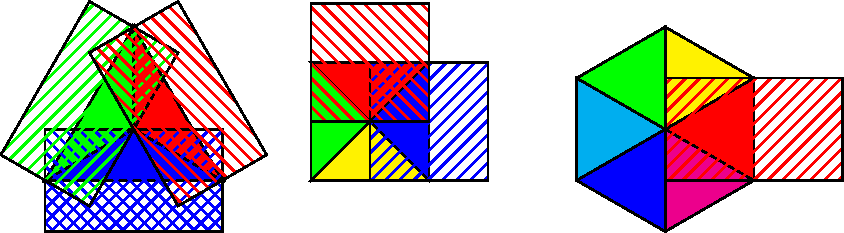
\includegraphics{fig_main_boxes.pdf}
\end{center}
\caption{Horizontal shapes of possible main grid boxes and examples of associated edge volumes.}
\label{tri_cont_vol}
\end{figure}

Look at Figure \ref{tri_cont_vol} and observe that each lateral interface
of the main grid box is represented by a rectangular domain. Each edge
velocity point has such an associated quadrilateral box as the local control
volume and possesses its local metrics which is required for the numerical computations
of the divergence (for the flux through the triangle interfaces) and
rotation operator (for the definition of the boundaries which enclose the
vortex lines in a certain direction). All the following derivations are in principle
suitable for triangular, hexagonal and quadrilateral grids.

We now add a third vertical dimension on the quadrilateral edge surfaces
in Figure \ref{cont_volu}. The three-dimensional edge control volume is
sketched with black lines. In the following, all numerical operators will be
defined using a similar three-dimensional box, but the box might be shifted in the
vertical to match with the actual local position where we need it.
We should be aware that the box may be inclined because of the varying terrain height.
The terrain height $z$ in the model turns out to be best defined at the centers of
the main box vertical interface points, that is where the vertical velocity $w$ is defined on
a Lorenz grid, {\it and} on the corners of these surfaces. Than, the slope of the
box may only be felt in two directions: namely that horizontal direction which connects the height points at the centers of the triangles, quadrilaterals or hexagons, which is later needed for the metric terms of the velocity fields, {\it and} that horizontal direction which connects the corner points, so that the metric terms are
later defined for the vortex vector fields.
As naming convention we refer to the former sloping direction with index
$\mathbf{n}$ as this direction is normal to the main box interfaces,
and to the latter horizontal direction with the index $\mathbf{t}$ as it is
tangential along the main box horizontal interfaces.

We follow now closely the textbook of Zdunkowski and Bott (2003) in defining
reciprocal coordinate systems that lead us through the derivations of all
essential differential operators. This concept exploits that any vector may be represented
with any kind of a linearly independent vector basis.
Two different vector bases chosen to possess certain 'reciprocal' properties
facilitate our derivations in particular.
To become familiar with that concept, we exemplarily draw the
covariant and contravariant base vectors
$\mathbf{q_i}$ and $\mathbf{q^i}$ in the center of the quadrilateral box in
Figure \ref{cont_volu}.
The covariant base vectors are defined to be tangential to the
coordinate lines, which are here defined as the lines connecting the height
points. As the contragredient (reciprocal) representation we
find the contravariant base vectors to be defined perpendicular to the coordinate surfaces,
which is achieved by the main definition of reciprocal coordinate systems
\begin{equation}
 \mathbf{q^i}\cdot\mathbf{q_k}=\delta_k^i.
\label{contragredient}
\end{equation}

\begin{figure}[t]
%\begin{pdfpic}
\setlength{\unitlength}{1cm}
\pspicture*(10,8)(-2,-1)
\psset{unit=1cm}
\psset{fillstyle=none}
\psline[linestyle=solid](0,0)(6,1)
\psline[linestyle=solid](6,1)(8,3)
\psline[linestyle=dashed](8,3)(2,2)
\psline[linestyle=dashed](2,2)(0,0)
\pspolygon[linestyle=solid](0,4)(6,5)(8,7)(2,6)
\psline[linestyle=solid](0,0)(0,4)
\psline[linestyle=solid](6,5)(6,1)
\psline[linestyle=solid](8,7)(8,3)
\psline[linestyle=dashed](2,2)(2,6)
\rput[B](0.8,3.2){$w, \dot{q}^z, \dot{q}_z$}
\rput[B](0.8,2.8){$z$}
\rput[B](2.8,2.4){$z$}
\rput[B](6.9,4.2){$w, \dot{q}^z, \dot{q}_z$}
\rput[B](7.2,3.8){$z$}
\rput[B](5.2,4.4){$z$}
\rput[B](0.6,5.0){$\varrho, \theta_v$}
\rput[B](0.6,1.0){$\varrho, \theta_v$}
\rput[B](7.5,2.0){$\varrho, \theta_v$}
\rput[B](7.5,6.0){$\varrho, \theta_v$}
\rput[B](4.2,1.2){$\dot{x}_n, \dot{q}^n, \dot{q}_n$}
\rput[B](4.0,5.6){$\dot{x}_n, \dot{q}^n, \dot{q}_n$}
\rput[B](-0.8,2.8){\tt l:=k-1/2}
\rput[Br](9.6,4.0){\tt l:=k-1/2}
\rput[B](8.2,2.0){\tt k}
\rput[B](-0.4,1.0){\tt k}
\rput[B](8.4,6.0){\tt k-1}
\rput[B](-0.4,5.0){\tt k-1}
\rput[b](-0.2,0.1){\tt i}
\rput[b](3.4,0.0){\tt j:=i+1/2}
\rput[b](6.0,0.1){\tt i+1}
\psset{linecolor=red}
\pspolygon[linestyle=dashed](3,0.5)(5,2.5)(1,1)
\pspolygon[linestyle=solid](3,4.5)(5,6.5)(1,5)
\psline[linestyle=solid](3,0.5)(3,4.5)
\psline[linestyle=dashed](5,2.5)(5,6.5)
\psline[linestyle=dashed](1,1)(1,5)
\psset{linecolor=gray,linestyle=dotted}
\pspolygon(3,0.5)(5,2.5)(7,2)
\pspolygon(3,4.5)(5,6.5)(7,6)
\psline(3,0.5)(3,4.5)
\psline(5,2.5)(5,6.5)
\psline(7,2)(7,6)
\psset{linecolor=green,linestyle=dotted}
\psline(1,5)(7,6)
\psline(1,1)(7,2)
\psset{linecolor=black}
\qdisk(1,3){2pt}
\qdisk(7,4){2pt}
\qdisk(4,5.5){2pt}
\qdisk(1,1){2pt}
\qdisk(7,2){2pt}
\qdisk(4,1.5){2pt}
\qdisk(7,6){2pt}
\qdisk(1,5){2pt}
\qdisk(5,4.5){2pt}
\qdisk(3,2.5){2pt}
\psline[linecolor=blue](1,3)(7,4)
\psline[linecolor=blue](4,1.5)(4,5.5)
\psline[linecolor=blue](3,2.5)(5,4.5)
\psset{linestyle=solid}
\psline[linecolor=blue,arrowscale=2]{->}(4,3.5)(5,3.6667)
\psline[linecolor=blue,arrowscale=2]{->}(4,3.5)(4,4.5)
\psline[linecolor=blue,arrowscale=2]{->}(4,3.5)(4.5,4)
\rput[B](5.2,3.8){\color{blue}$\mathbf{q_n}$}
\rput[B](4.3,4.4){\color{blue}$\mathbf{q_z}$}
\rput[B](4.7,4.1){$\mathbf{{\color{gray}q}^{\color{green}t}_{\color{blue}t}}$}
\psline[linecolor=green,arrowscale=2]{->}(4,3.5)(5,3.5)
\psline[linecolor=green,linestyle=dashed](4,3.5)(4.5,4)
\psline[linecolor=green,arrowscale=2]{->}(4,3.5)(3.85,4.4)
\rput[B](5.2,3.3){\color{green}$\mathbf{q^n}$}
\rput[B](3.6,4.3){\color{green}$\mathbf{q^z}$}
\endpspicture
\end{pdfpic}


\begin{center}
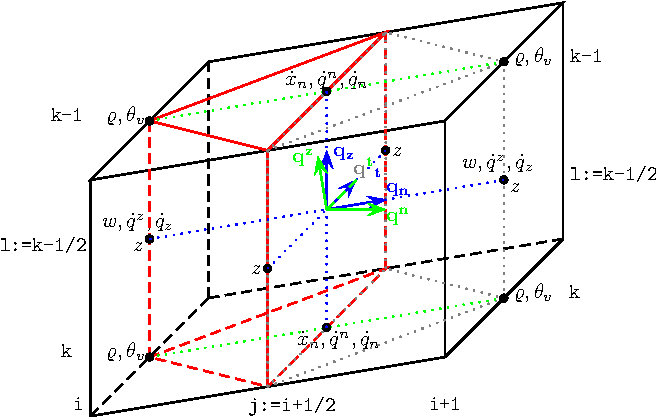
\includegraphics{fig_edge_volume.pdf}
\end{center}
\caption{Example of a 3 dimensional control volume element}
\label{cont_volu}
\end{figure}

As we do our measurements of actual heights, winds and vorticities in an orthogonal
spherical coordinate system attached to the Earth we need a relationship
between the orthogonal unit base vectors
$\mathbf{e}_{\lambda},\mathbf{e}_{\phi},\mathbf{e}_r$ and the covariant and
contravariant base vectors attached to a local terrain-following coordinate system.
We assume here, that the first step in that coordinate transformation has already
achieved, namely that part, that converts horizontal spherical unit vectors to orthogonal
unit vectors at the lateral interfaces of the main grid boxes. Thus, we assume to have
already access to orthogonal unit vectors $\mathbf{e_n}$ and $\mathbf{e_t}$ at
the mentioned positions. The second step of the transformation is thus introduced in the
following. The coordinate surfaces in the covariant coordinate system are naturally given
as surfaces with constant contravariant measure numbers $q^i$. The vertical surfaces of constant $q^n=x_n$ and $q^t=x_t$ do not change when changing from the
orthogonal to the terrain following coordinate system. The horizontal surface of
constant vertical contravariant coordinate $q^z$
\begin{displaymath}
 q^z=q^z(x_n,x_t,z)
\end{displaymath}
crosses the horizontal surface of constant $z$ in the orthogonal coordinate system.
The gradient of the contravariant coordinate surfaces is perpendicular to surfaces of constant $q^i$ and gives thus the contravariant base vectors
\begin{displaymath}
 \mathbf{q^i}=\nabla q^i.
\end{displaymath}
By employing the gradient in the orthogonal system as $\nabla=\mathbf{e_n}\partial_{x_n}+\mathbf{e_t}\partial_{x_t}+\mathbf{e_z}\partial_z$
and (\ref{contragredient}) we observe the following relationships
\begin{equation}
\begin{array}{lll}
\mathbf{q^n}=\mathbf{e_n}\qquad\qquad\qquad&
\mathbf{q^t}=\mathbf{e_t}\qquad&
\mathbf{q^z}=\frac{\partial q^z}{\partial z}\mathbf{e_z}+\frac{\partial q^z}{\partial x_n}\mathbf{e_n}
                +\frac{\partial q^z}{\partial x_t}\mathbf{e_t}      \\
\mathbf{q_n}=\mathbf{e_n}+\frac{\partial z}{\partial x_n}\mathbf{e_z}\qquad&
\mathbf{q_t}=\mathbf{e_t}+\frac{\partial z}{\partial x_t}\mathbf{e_z}\qquad&
\mathbf{q_z}=\frac{\partial z}{\partial q^z}\mathbf{e_z}\\
\mathbf{e_n}=\mathbf{q_n}+\frac{\partial q^z}{\partial x_n}\mathbf{q_z}\qquad&
\mathbf{e_t}=\mathbf{q_t}+\frac{\partial q^z}{\partial x_t}\mathbf{q_z}\qquad&
\mathbf{e_z}=\frac{\partial q^z}{\partial z}\mathbf{q_z}\\
\mathbf{e_n}=\mathbf{q^n}\qquad\qquad\qquad&
\mathbf{e_t}=\mathbf{q^t}\qquad&
\mathbf{e_z}=\frac{\partial z}{\partial q^z}\mathbf{q^z}+\frac{\partial z}{\partial x_n}\mathbf{q^n}
+\frac{\partial z}{\partial x_t}\mathbf{q^t}
\end{array}
\end{equation}
Additionally, we find the functional determinant of the system as
\begin{displaymath}
 \sqrt{g}=[\mathbf{q_n},\mathbf{q_t},\mathbf{q_z}]=\mathbf{q_n}\cdot
(\mathbf{q_t}\times\mathbf{q_z})=\frac{\partial z}{\partial q^z}\Rightarrow \mathbf{q^n}=\frac{1}{\sqrt{g}}\mathbf{q_t}\times
\mathbf{q_z}.
\end{displaymath}
General volumes and covariant areas are given by
\begin{eqnarray*}
 d\tau &= &\sqrt{g}dq^ndq^tdq^z\\
 ds_n&=&\sqrt{g}dq^tdq^z\\
 ds_t&=&\sqrt{g}dq^ndq^z\\
 ds_z&=&\sqrt{g}dq^ndq^t,
\end{eqnarray*}
other important measures are the two terrain slopes, that we abbreviate with $J_n=\partial z/\partial x_n$ and $J_t=\partial z/\partial x_t$, respectively.

We may now express the velocity vector in the three different coordinate systems by using the relationships so far. In the C-grid, only normal velocity components are available. Tangential winds may not directly be accessed, and thus play no role for the current step of our description.
\begin{eqnarray*}
 \mathbf{v}&=&\dot{x}_n\mathbf{e_n}+w\mathbf{e_z}\\
 \mathbf{v}&=&\dot{x}_n\mathbf{q_n}+
              \frac{\partial q^z}{\partial z}(w-\dot{x}_n\frac{\partial z}{\partial x_n})\mathbf{q_z}\\
           &=&\dot{q}^n\mathbf{q_n}+\dot{q}^z\mathbf{q_z}\\
 \mathbf{v}&=&(\dot{x}_n+w\frac{\partial z}{\partial x_n})\mathbf{q^n}
              +w\frac{\partial z}{\partial q^z}\mathbf{q^z}\\
           &=&\dot{q}_n\mathbf{q^n}+\dot{q}_z\mathbf{q^z}
\end{eqnarray*}
Here, $\dot{q}^i$ are called the contravariant wind components,
$\dot{q}_i$ are referred to as the covariant wind components and
$\dot{x}_n,\dot{x}_t,w$ denote the orthogonal wind components.

For the representation of the vorticity vector, we encounter the opposite situation: normal components are not needed, rather the tangential vorticity components are automatically given in the C-grid
\begin{eqnarray*}
 \vec{\omega}&=&\dot{\xi}_t\mathbf{e_t}+\dot{\xi_z}\mathbf{e_z}\\
 \vec{\omega}&=&\dot{\xi}_t\mathbf{q_t}+
                \frac{\partial q^z}{\partial z}(\dot{\xi}_z
                -\dot{\xi}_t\frac{\partial z}{\partial x_t})\mathbf{q_z}\\
             &=&\dot{\omega}^t\mathbf{q_t}+\dot{\omega}^z\mathbf{q_z}\\
 \vec{\omega}&=&(\dot{\xi}_t+\dot{\xi}_z\frac{\partial z}{\partial x_t})\mathbf{q^t}
                +\dot{\xi}_z\frac{\partial z}{\partial q^z}\mathbf{q^z}\\
             &=&\dot{\omega}_t\mathbf{q^t}+\dot{\omega}_z\mathbf{q^z}
\end{eqnarray*}

Later, we need some transformations between the covariant, contravariant and orthogonal measure numbers
\begin{equation}
\begin{array}{lll}
\dot{q}^n=\dot{x}_n&
\dot{q}_n=\dot{x}_n+wJ_n&
\dot{\xi}_t=\dot{\omega}^t\\
\dot{q}^z=\left(w-\dot{x}_nJ_n\right)/\sqrt{g}&
\dot{q}_z=w\sqrt{g}&
\dot{\xi}_z=\dot{\omega}^z\sqrt{g}+\dot{\omega}^tJ_t
\end{array}
\label{conversions}
\end{equation}
At the moment, these expressions are to be regarded as symbolically written because there is no position in the grid where those relationships may be taken literally.

Closing this first section we mention the geometric
measures needed in our model as the horizontal distance between the box midpoints: the dual arc lengths
$\delta=dq^n$, the length of the edges: the primal arc lengths $\lambda=dq^t$, and the vertical distance
between two main grid box centers $\Delta z=\sqrt{g}$, so that $dq^z=1$. From now on, all differentials will be used as finite differences in our manuscript. 

Before we devote ourselves to the numerical operators on the grid, the labeling of the grid points should
be introduced as alredy indicated in Figure \ref{cont_volu}. For convenience with traditional modeling style, the index counter increases from to to bottom. The vertical labels of the grid points are
denoted with $k$ for entities in vertical layers (full levels) and the conventional indexing of the upper adjacent interface height (half levels) $k-1/2$ will in the following be replaced by $l^-$. The main grid boxes are counted with the index $i$ and the lateral interface positions conventionally labeled with
$i+1/2$ labels will be counted with $j$ indices. When referring to the lateral faces of a grid box we write $j\in i$, and when referring to the top/bottom faces we use the $l\in k$ notation.

\section{Divergence operator}

The divergence of a flux $\mathbf{F}=\psi\varrho\mathbf{v}$ is given by the Gauss theorem
\begin{displaymath}
 \int_V\nabla\cdot\mathbf{F}d\tau = \int_S\mathbf{F}\cdot d\mathbf{s}.
\end{displaymath}
When computing this on a numerical grid, the RHS and LHS are determined at different positions (center and interfaces), and take advantage of the character of the contragredient coordinate systems
\begin{eqnarray}
 d\tau_{i,k}\nabla\cdot\mathbf{F} &=&
\left[\sum_{j\in i}f^{n,j}\mathbf{q_{n,j}}\cdot ds_{n,j}\mathbf{q^{n,j}}\right]_k
+\left[\sum_{l\in k}f^{z,l}\mathbf{q_{z,l}}\cdot ds_{z,l}\mathbf{q^{z,l}}\right]_i\nonumber\\
&=&\left[\sum_{j\in i}f^{n,j} ds_{n,j}\right]_k+\left[\sum_{l\in k}f^{z,l} ds_{z,l}\right]_i.
\label{divergence}
\end{eqnarray}
\begin{itemize}
 \item {\bf The LHS refers to the main grid box} (either triangular, quadrilateral or hexagonal) with
 $$d\tau_{i,k} = A_{i,k}\sqrt{g}_{i,k}dq^z=A_{i,k}\sqrt{g}_{i,k}.$$ The horizontal area $A_{i,k}$
 is formed by the summation of the subtriangle areas shown in Figure \ref{tri_cont_vol} at the layer
 height
 $$z_{i,k}=({z_{i,l^+}+z_{i,l^-}})/2,$$ which is by definition the arithmetic mean of the two adjacent
 level heights. This philosophy was already pursued in the COSMO. The thickness of the box is given by
 $$\sqrt{g}_{i,k}=z_{i,l^-}-z_{i,l^+}>0.$$
 \item {\bf The RHS refers to the grid box interfaces.}\\
Here we pose the question on how much air leaves the main grid box through the interfaces.
As the associated outwards pointing surface vectors $d\mathbf{s}$ are then required with contravariant base vectors (cf.~Figure \ref{cont_volu}) and thus covariant measure numbers, we need according to (\ref{contragredient}) contravariant measure numbers for the representation of the flux $\mathbf{F}$.
Let us now distinguish lateral interfaces $j$ and bottom/top interfaces $l$
 \begin{itemize}
   \item {\bf lateral interfaces}, where the normal components $n$ of the velocity (or flux) are defined
         \begin{displaymath}
         f^{n,j}ds_{n,j(i)} = f^{n,j}\overline{\sqrt{g}}^jdq^zdq^{t,j}\gamma_{j(i)}=
                              f^{n,j}\overline{\sqrt{g}}^jdq^{t,j}\gamma_{j(i)}
         \end{displaymath}
         Note here that the horizontal averaging is not automatically a one half weighting if the grid is
         not equilateral in the horizontal
         \begin{displaymath}
         \overline{\sqrt{g}}^j=\frac{1}{dq^{n,j}}\sum_{i\in j}\sqrt{g}_i
                                   \widetilde{dq}^{n,i(j)}
         \end{displaymath}
         where the $\widetilde{\;\;}$ indicates that the distances between the main box midpoint and the
         interface are measured.
         We have to consider furthermore the local outward
         normal direction with respect to both adjacent main boxes by means of 
         $$|\gamma_{j(i)}|=1\qquad\qquad \sum_{i\in j}\gamma_{i(j)}=0.$$
         $\gamma$ takes a positive or negative sign depending on whether the wind component points
         locally outwards or inwards with respect to the main box.\\
         The contravariant velocity measure number $\dot{q}^n$ as defined in (\ref{conversions}) is
         to be obtained from the orthogonal components without further additional computations, $\dot{q}^n=\dot{x}_n$.
   \item {\bf top/bottom interfaces}
         \begin{equation}
         f^{z,l}ds_{z,l} = f^{z,l}\overline{\sqrt{g}}^lA_{l}\gamma_{l(k)}
         \label{vertflux}
         \end{equation}
         According to the mentioned concept that the layer heights are the arithmetic means from the
         interface levels, the height averaging in the previous formula is
         $$\overline{\sqrt{g}}^l=\sum_{k\in l}\sqrt{g}_{k}/2.$$
         Differently from the lateral interface case, the definition of the inward and outward direction
         is simpler: $\gamma_{l(k)}$ is positive when used as the top interface and negative when used as
         the bottom interface, because we use a positive upward coordinate direction everywhere.\\
         The contravariant vertical velocity as defined in (\ref{conversions}) must be obtained by some
         transformational computations, using the definition of the inner product on the triangular, quadrilateral or
         hexagonal mesh
         \begin{equation}
          \dot{q}^{z,i,l} =[(w-x_nJ_n)/\sqrt{g}]_{i,l}=
                     \left(w_{i,l}-\overline{\frac{1}{A_{i,k}}\sum_{j\in i}
                     \dot{x}_{n,j,k}J_{n,j,k}\widetilde{dq}^{n,j(i),k}dq^{t,j,k}}^l\right)/\overline{\sqrt{g}}^l_{i,l},
         \label{contrav_velo}
         \end{equation}
         where the metric term is vertically averaged and given as
         \begin{equation}
          \overline\psi^l=\frac{1}{\overline{\sqrt{g}}^lA_l}\sum_{k\in l}\frac{\sqrt{g}_k}{2} A_k \psi_k.
         \label{avel}
         \end{equation}

 \end{itemize}
\end{itemize}

\section{Hamiltonian, functional derivatives and Poisson brackets\label{poisson}}
As already introduced in the previous chapter, we want to pose our problem on the Poisson structure of the dynamics. Thus, we first have to specify the
Hamiltonian using the orthogonal measure numbers for the velocity. It reads
\begin{eqnarray*}
 \mathcal{H}&=&\sum_{i,k}\varrho_{i,k}
             \left(\Phi_{i,k}+c_{vd}T_{i,k}+\right.\\
&&\left.\frac{1}{A_{i,k}\sqrt{g}_{i,k}}\left(
             \sum_{j\in i} \widetilde{dq}^{n}_{j(i),k}dq^{t}_{j,k}\overline{\sqrt{g}}^j_{j,k}
             \frac{\dot{x}_{n,j,k}^2}{2} +
             \sum_{l\in k} A_{i,l}\frac{\sqrt{g}_{i,k}}{2}
             \frac{w_{i,l}^2}{2}
             \right)\right)A_{i,k}\sqrt{g}_{i,k}\\
\mathcal{H}&=&\sum_{i,k}\varrho_{i,k}(\Phi_{i,k}+c_{vd}T_{i,k}+K_{i,k})A_{i,k}\sqrt{g}_{i,k}
\end{eqnarray*}
in which the definition of the specific kinetic energy $K_{i,k}$ becomes obvious.
We may rewrite the kinetic energy part of the Hamiltonian as to be built up from a sum over all $j$ and $l$ interfaces
\begin{displaymath}
 \mathcal{H}_{kin}=\sum_{j,k} {dq}^{n}_{j,k}dq^{t}_{j,k}\overline{\sqrt{g}}^j_{j,k}\bar{\varrho}^{j}_{j,k}
             \frac{\dot{x}_{n,j,k}^2}{2} +
             \sum_{i,l} A_{i,l}\overline{\sqrt{g}}^l_{i,l}
             \frac{w_{i,l}^2}{2}\bar{\varrho}^{l}_{i,l}
\end{displaymath}
Performing this transformation we find immediately the averaging rules for the density to the interfaces
\begin{displaymath}
 \bar{\varrho}^j_{j,k} = \frac{1}{dq^n_{j,k}}\sum_{i\in j}\varrho_{i,k}\widetilde{dq}^n_{i(j),k}
\qquad\qquad\qquad
 \bar{\varrho}^l_{i,l} = \frac{1}{\overline{\sqrt{g}}^l_{i,l}}\sum_{k\in l}\varrho_{i,k}\frac{\sqrt{g}_{i,k}}{2}.
\end{displaymath}
Note, that those averaging rule is not exactly equivalent to the averagings
introduced for $\sqrt{g}$ or for the metric term in (\ref{avel}).

Further, we need functional derivatives with respect to the orthogonal measure numbers, which can be easily found to give
\begin{displaymath}
 \frac{\delta\mathcal{H}}{\delta \dot{x}_n}=\bar{\varrho}^j \dot{x}_n\qquad\qquad\qquad
 \frac{\delta\mathcal{H}}{\delta w}=\bar{\varrho}^l w.
\end{displaymath}
The other functional derivatives needed for the Poisson bracket evaluations do not touch vectors and thus
yield the same results as in the continuous case
\begin{displaymath}
 \frac{\delta\mathcal{H}}{\delta\varrho}=K+\Phi\qquad\qquad\qquad
 \frac{\delta\mathcal{H}}{\delta\tilde\theta_v}=c_{pd}\Pi.
\end{displaymath}
The Poisson brackets for our dynamical problem are written as
\begin{eqnarray}
 \{\mathcal{F},\mathcal{H}\}_{\varrho}&=&-\sum_{i,k}\left(
     \frac{\delta\mathcal{F}}{\delta \varrho}\nabla\cdot\frac{\delta\mathcal{H}}{\delta\mathbf{v}}-
     \frac{\delta\mathcal{H}}{\delta \varrho}\nabla\cdot\frac{\delta\mathcal{F}}{\delta\mathbf{v}}
     \right)_{i,k} A_{i,k}\sqrt{g}_{i,k}
\label{eqn_poiss1}\\
\{\mathcal{F},\mathcal{H}\}_{\tilde\theta_v}&=&-\sum_{i,k}\left(
\frac{\delta\mathcal{F}}{\delta\tilde\theta_{v}}\nabla\cdot
\left(\theta_v\frac{\delta\mathcal{H}}{\delta\mathbf{v}}\right)-
\frac{\delta\mathcal{H}}{\delta\tilde\theta_{v}}\nabla\cdot
\left(\theta_v\frac{\delta\mathcal{F}}{\delta\mathbf{v}}\right)
     \right)_{i,k} A_{i,k}\sqrt{g}_{i,k}
\label{eqn_poiss2}
\end{eqnarray}
for arbitrary $\mathcal{F}$. If we choose $\mathcal{F}$ as to represent Delta functionals of local
values of the prognostic variables, we find
\begin{eqnarray*}
 \frac{\delta(\mathcal{F}=\dot{x}_{n,j1,k1})}{\delta\dot{x}_n}&=&
                          \frac{1}{dq^{n,j1,k1}dq^{t,j1,k1}\overline{\sqrt{g}}^j_{j1,k1}}
                          \mbox{ if } j1=j \mbox{ and } k1=k\\
                          &=&0 \mbox{ otherwise }\\
 \frac{\delta(\mathcal{F}=w_{i1,l1})}{\delta w}&=&
                          \frac{1}{A_{i1,l1}\overline{\sqrt{g}}^l_{i1,l1}}
                          \mbox{ if } i1=i \mbox{ and } l1=l\\
                          &=&0 \mbox{ otherwise }\\
 \frac{\delta(\mathcal{F}=\varrho_{i1,k1})}{\delta\varrho}&=&
                          \frac{1}{A_{i1,k1}\sqrt{g}_{i1,k1}}
                          \mbox{ if } i1=i \mbox{ and } k1=k\\
                          &=&0 \mbox{ otherwise }\\
\frac{\delta(\mathcal{F}=\tilde\theta_{v,i1,k1})}{\delta\tilde\theta_v}&=&
                          \frac{1}{A_{i1,k1}\sqrt{g}_{i1,k1}}
                          \mbox{ if } i1=i \mbox{ and } k1=k\\
                          &=&0 \mbox{ otherwise }.
\end{eqnarray*}

\section{Gradient operator}
From the definition of the divergence and the Poisson bracket, we may now derive the gradient operator,
which is the dual of the divergence. The vertical gradients needed in the vertical velocity equation are
found if $\mathcal{F}=w_{i1,l1}$ is inserted into both Poisson brackets, (\ref{eqn_poiss1}) and
(\ref{eqn_poiss2}). For the example (\ref{eqn_poiss1}) we find by using (\ref{divergence}), (\ref{vertflux}) and (\ref{contrav_velo})
\begin{eqnarray*}
\{\mathcal{F}=w_{i1,l1},\mathcal{H}\}_\varrho&=&
\sum_{i,k}\frac{\delta\mathcal{H}}{\delta\varrho}_{i,k}\sum_{l\in k}A_{i,l}\gamma_{i,l(k)}
\frac{\delta\mathcal{F}}{\delta w}_{i,l}\\
\{\mathcal{F}=w_{i1,l1},\mathcal{H}\}_\varrho&=&
\sum_{i,l}A_{i,l}\frac{\delta\mathcal{F}}{\delta w}_{i,l}\sum_{k\in l}\gamma_{i,k(l)}K_{i,k}\\
\{\mathcal{F}=w_{i1,l1},\mathcal{H}\}_\varrho&=&-\frac{K_{i1,k1-1}-K_{i1,k1}}{\overline{\sqrt{g}}^l_{i1,l1}}
=-\partial_zK
\end{eqnarray*}
A similar derivation is found for the contribution of the Poisson bracket (\ref{eqn_poiss2})
\begin{displaymath}
 \{\mathcal{F}=w_{i1,l1},\mathcal{H}\}_{\tilde\theta_v}=-c_{pd}\hat{\theta}^l_{v,i,l}\partial_z\Pi,
\end{displaymath}
where the actual vertical reconstruction of $\hat{\theta}^l_{v,i,l}$ is left open at the moment, it will be defined later
in the advection scheme for scalars.

The horizontal gradient operator contains also a metric correction term, 
which stems from the contravariant correction part in (\ref{contrav_velo}) 
of the divergence
\begin{eqnarray*}
 \{\mathcal{F}=\dot{x}_{n,j1,k1},\mathcal{H}\}_\varrho&=&
\sum_{i,k}\frac{\delta\mathcal{H}}{\delta\varrho}_{i,k}\sum_{j\in i}\frac{\delta\mathcal{F}}{\delta \dot{x}_n}_{j,k}
\overline{\sqrt{g}}^j_{j,k}dq^{t,j,k}\gamma_{j(i),k}\\&&
-\sum_{i,k}\frac{\delta\mathcal{H}}{\delta\varrho}_{i,k}
\sum_{l\in k}\gamma_{i,l(k)}\frac{1}{\overline{\sqrt{g}}^l_{i,l}}\sum_{k\in l}\frac{\sqrt{g}_{i,k}}{2}\sum_{j\in i}
\frac{\delta\mathcal{F}}{\delta \dot{x}_n}_{j,k} J_{n,j,k}\widetilde{dq}^{n,j(i),k}dq^{t,j,k}\\
 \{\mathcal{F}=\dot{x}_{n,j1,k1},\mathcal{H}\}_\varrho&=&
\sum_{j,k}\frac{\delta\mathcal{F}}{\delta \dot{x}_n}_{j,k}\overline{\sqrt{g}}^j_{j,k}dq^{t,j,k}\sum_{i\in j}
K_{i,k}\gamma_{i(j),k}\\&&
-\sum_{j,k}\frac{\delta\mathcal{F}}{\delta \dot{x}_n}_{j,k}J_{n,j,k}dq^{t,j,k}
\sum_{i\in j}\widetilde{dq}^{n,i(j),k}\frac{\sqrt{g}_{i,k}}{2}
\sum_{l\in k}\frac{1}{\overline{\sqrt{g}}^l_{i,l}}
\sum_{k\in l}\gamma_{i,k(l)}K_{i,k}\\
\{\mathcal{F}=\dot{x}_{n,j1,k1},\mathcal{H}\}_\varrho&=&\frac{1}{dq^{n,j1,k1}}\sum_{i\in j1}K_{i,k1}\gamma_{i(j1),k1}\\
&&-\frac{J_{n,j1,k1}}{dq^{n,j1,k1}\overline{\sqrt{g}}^j_{j1,k1}}
\sum_{i\in j1}\widetilde{dq}^{n,i(j1),k1}\frac{\sqrt{g}_{i,k1}}{2}
\sum_{l\in k1}\frac{1}{\overline{\sqrt{g}}^l_{i,l}}
\sum_{k\in l}\gamma_{i,k(l)}K_{i,k}\\
\{\mathcal{F}=\dot{x}_{n,j1,k1},\mathcal{H}\}_\varrho&=&
-\partial_{n}K+J_n\overline{\overline{\partial_zK}^k}^j
\end{eqnarray*}
From this result, we derive vertical
\begin{equation}
        \overline{\psi}^k=\sum_{l\in k}\frac{1}{2}\psi_l,
       \label{avek}
\end{equation}
and horizontal averaging rules
\begin{equation}
        \overline{\psi}^j=\frac{1}{dq^{n,j}\overline{\sqrt{g}}^j_{j}}\sum_{i\in j}
        \sqrt{g}_i\widetilde{dq}^{n,i(j)}\psi_i
       \label{avej}
\end{equation}
for general scalars. The horizontal pressure gradient term defined via (\ref{eqn_poiss2}) yields via a similar procedure
\begin{displaymath}
 \{\mathcal{F}=\dot{x}_{n,j1,k1},\mathcal{H}\}_{\tilde\theta_v}=
-c_{pd}\hat{\theta}^j\partial_{n}\Pi+J_nc_{pd}\overline{\overline{\hat\theta^l\partial_z\Pi}^k}^j,
\end{displaymath}
where the already known averaging rules (\ref{avek}) and (\ref{avej}) apply.

\section{Rotation operator}

To compute the rotation of a vector, we originate from the Gauss theorem and assume that the flux vector
$\mathbf{F}$ could have been obtained by the vector multiplication of two vectors
$\mathbf{F}=\nabla q^i\times\mathbf{v}$. That yields
\begin{eqnarray*}
 \int_V\nabla\cdot\mathbf{F}d\tau&=&\int_S\mathbf{F}\cdot d\mathbf{s}\\
 \int_V\nabla\cdot(\nabla q^i\times\mathbf{v})d\tau&=&\int_S(\nabla q^i\times\mathbf{v})\cdot d\mathbf{s}\\
 \int_V[-\nabla q^i\cdot(\nabla\times\mathbf{v})
       +\mathbf{v}\cdot(\nabla\times\nabla q^i)]d\tau&=&\int_S(\nabla q^i\times\mathbf{v})\cdot d\mathbf{s}\\
 \int_V-\nabla q^i\cdot(\nabla\times\mathbf{v})d\tau&=&\int_S(\nabla q^i\times\mathbf{v})\cdot d\mathbf{s}\\
 \int_V-\mathbf{q^i}\cdot(\nabla\times\mathbf{v})d\tau&=&\int_S(\mathbf{q^i}\times\mathbf{v})\cdot d\mathbf{s}\\
 \int_V\mathbf{q^i}\cdot(\nabla\times\mathbf{v})d\tau&=&-\int_S(\mathbf{q^i}\times\mathbf{v})\cdot d\mathbf{s}\\
 \int_V\mathbf{q^i}\cdot(\nabla\times\mathbf{v})d\tau&=&\int_S\mathbf{v}\cdot(\mathbf{q^i}\times d\mathbf{s})
\end{eqnarray*}
From the RHS we recognise that the outward pointing $d\mathbf{s}=\sum_ids_i\mathbf{q^i}$ is a vector in the contravariant system. Thus, $\mathbf{v}=\sum_i \dot{q}_i \mathbf{q^i}$ is also needed in that system so as to evaluate the scalar triple product most easily. The resulting vector $\nabla\times\mathbf{v}$ on the LHS comes in the covariant system as $\vec{\omega}=\sum_i\omega^i\mathbf{q_i}$. Significant contributions to the RHS occur
only for specific $\mathbf{q^i}$ if the vector product does not vanish and points into a direction
for that we have a vector component of $\mathbf{v}$ available:
\begin{eqnarray*}
 \mathbf{q^z}\times ds_t\mathbf{q^t}&=&-ds_t\mathbf{q_n}/\sqrt{g}\\
 \mathbf{q^t}\times ds_n\mathbf{q^n}&=&-ds_n\mathbf{q_z}/\sqrt{g}\\
 \mathbf{q^t}\times ds_z\mathbf{q^z}&=&ds_z\mathbf{q_n}/\sqrt{g}
\end{eqnarray*}
These three cases will now be investigated separately
\begin{itemize}
 \item $\mathbf{q^z}\times ds_t\mathbf{q^t}$: Then, the RHS integral contributions become
       \begin{displaymath}
        \mathbf{v}\cdot(\mathbf{q^z}\times ds_t\mathbf{q^t})=-\dot{q}_n\mathbf{q^n}\cdot\mathbf{q_n} ds_t/\sqrt{g}
        =-\dot{q}_n\; dq^ndq^z=-\dot{q}_n\; dq^n
       \end{displaymath}
       which are summed up for the dual horizontal grid $m$ which is a hexagon/pentagon if the main
       grid box has triangular shape and a rhombus, if the main grid box has hexagonal shape. Finally, the
       contravariant vertical vorticity is obtained via
       \begin{displaymath}
        \omega^{z}_{m,k}=\frac{1}{A_{m,k}\overline{\sqrt{g}}^m_{m,k}}
        \sum_{j \in m}\dot{q}_{n;j,k}\; dq^{n,j,k}\gamma_{j(m),k}
       \end{displaymath}
       where $\gamma_{j(m),k}$ gives the sign convention for the positive mathematical sense.
       The area $A_{m,k}$
       is again determined by summing up the subtriangles forming the dual surface.
       The $\overline{\sqrt{g}}^m$
       averaging an arbitrary area weighting. This volumar measure appears here at the
       first glance unexpectedly, as we would have anticipated to divide only by an area.
       But if we transform the contravariant $\omega^{z}$ into an orthogonal measure according to
       (\ref{conversions}), this weighting disappears again.\\
       As the normal covariant measure numbers enter the computation of the contravariant vorticity
       component, we have to specify them via (\ref{conversions})
       \begin{displaymath}
        \dot{q}_{n,j,k}=[\dot{x}_n+wJ_n]_{j,k}=\dot{x}_{n,j,k}+
                        \overline{\overline{w_{i,l}}^k}^jJ_{n,j,k},
       \end{displaymath}
       where the previously derived vertical (\ref{avek}) and horizontal (\ref{avej}) averaging rules apply.
 \item $\mathbf{q^t}\times ds_n\mathbf{q^n}$: Then, the RHS integral contributions become
       \begin{displaymath}
        \mathbf{v}\cdot(\mathbf{q^t}\times ds_n\mathbf{q^n})=-\dot{q}_z\mathbf{q^z}\cdot \mathbf{q_z}ds_n/\sqrt{g}
        =-\dot{q}_z\; dq^tdq^z=-\dot{q}_z\; dq^t.
       \end{displaymath}
       Note, the surface measure invoked here calls for vertical slices positioned with their centers at the
       vertical velocity (height) points. But there, we only have information about their vertical extents, but not
       about their horizontal lengths $dq^t$. Thus, we must assume that each $dq^t$ at the height points is the
       same as at the horizontal
       interface between the two considered height points. Finally, the prorated rotation contribution at $j,l$ is
       \begin{displaymath}
        \omega^{t}_{j,l}=\frac{1}{dq^t dq^n_{j,l}\overline{\sqrt{g}}^{j,l}_{j,l}}\sum_{i\in j }\dot{q}_{z;i,l}dq^t
       \gamma_{i(j),l} = \frac{1}{dq^n_{j,l}\overline{\sqrt{g}}^{j,l}_{j,l}}\sum_{i\in j }\dot{q}_{z;i,l}
       \gamma_{i(j),l}
       \end{displaymath}
       where $\gamma_{i(j),l}$ gives the sign convention for the positive mathematical sense. Naturally
       the covariant vertical wind component is given by $\dot{q}_{z,i,l}=w_{i,l}\overline{\sqrt{g}}^{l}_{i,l}$.
 \item $\mathbf{q^t}\times ds_z\mathbf{q^z}$: Then, the RHS integral contributions become
       \begin{displaymath}
       \mathbf{v}\cdot(\mathbf{q^t}\times ds_z\mathbf{q^z})=\dot{q}_n\mathbf{q^n}\cdot\mathbf{q_n}ds_z/\sqrt{g}=
       \dot{q}_n dq^tdq^n
       \end{displaymath}
       Here, the areas $ds_z$ may be different at different height and we may not cancel any of the lengths
       involved. Thus, the prorated contribution to the rotation at $j,l$ yields
       \begin{displaymath}
        \omega^{t}_{j,l}=\frac{1}{dq^t_{j,l}dq^n_{j,l}\overline{\sqrt{g}}^{j,l}_{j,l}}\sum_{k\in l }\dot{q}_{n;j,k}
       dq^n_{j,k}dq^t_{j,k}
       \gamma_{j,k(l)}
       \end{displaymath}
       where $\gamma_{j,k(l)}$ gives the sign convention for the positive mathematical sense.
\end{itemize}
The last two points together give the full tangential vorticity component
\begin{displaymath}
\omega^{t}_{j,l}=\frac{1}{dq^n_{j,l}\overline{\sqrt{g}}^{j,l}_{j,l}}\sum_{i\in j }\dot{q}_{z;i,l}
\gamma_{i(j),l}+\frac{1}{dq^t_{j,l}dq^n_{j,l}\overline{\sqrt{g}}^{j,l}_{j,l}}\sum_{k\in l }
\dot{q}_{n;j,k}dq^n_{j,k}dq^t_{j,k}\gamma_{j,k(l)}.
\end{displaymath}
Later, if we want to evaluate the  vorticity flux term, we need the orthogonal vorticities according
to (\ref{conversions}). The horizontal component does not need a transformational calculation, but
the vertical vorticity component required the calculation of
\begin{displaymath}
{\xi}_{z,m,k}=[\sqrt{g}\omega^z+\omega^tJ_t]_{m,k}=\sqrt{g}_{m,k}\omega^{z,m,k}+
\overline{ \frac{1}{A_{m,l}}\sum_{j\in m}\omega^{t,j,l}J_{t,j,l}dq^{n,j,l}\widetilde{dq}^{t,j(m),l}}^k.
\end{displaymath}
